\documentclass{cubeamer}

\usepackage[french]{babel}
\usepackage[T1]{fontenc}
\usepackage{graphicx}

\title{Protection et gestion des licences}
\subtitle{Présentation - Gestion de projet}
\author{Sami Babigeon, Louka Boivin, Kaci Hammoudi, Alexis Osmont}
\date{\today}
\institute[Université de Rouen]{Master Informatique - 1ère année}

\begin{document}

\maketitle

\cutoc

%   Exemple de plan de présentation (mail de Karim)
%
%   Présentation du sujet et compréhension du besoin client
%   Périmètre fonctionnel à couvrir, appuyé par le diagramme global des cas d’utilisation
%   Solution technique argumentée avec diagramme d’architecture logicielle
%   Stratégie qualité pour la validation des livrables
%   Organisation du projet (i.e. affectation des rôles + découpage des tâches + stratégie de réalisation + organisation agile)
%   Planning du projet (i.e. focus sur les itérations > zoom sur le Gantt)
%   Principaux risques du projet et crédibilité de l'organisation mise en oeuvre
%
%   + POC si on a réussi

\section{Présentation du sujet}

\begin{frame}{Intitulé}
    \centerline{\textbf{Protection et gestion des licences}}
    \medskip
    \pause
    \emph{Objectifs :}
    \pause
    \begin{itemize}
        \item Génération et vérification des licences
        \pause
        \item Plateforme de gestion pour le client, de demande pour les utilisateurs
        \pause
        \item Protection des logiciels du client
    \end{itemize}
\end{frame}

\section{Analyse fonctionnel}

\begin{frame}{Cas d'utilisations}
    \begin{figure}
        \centering
        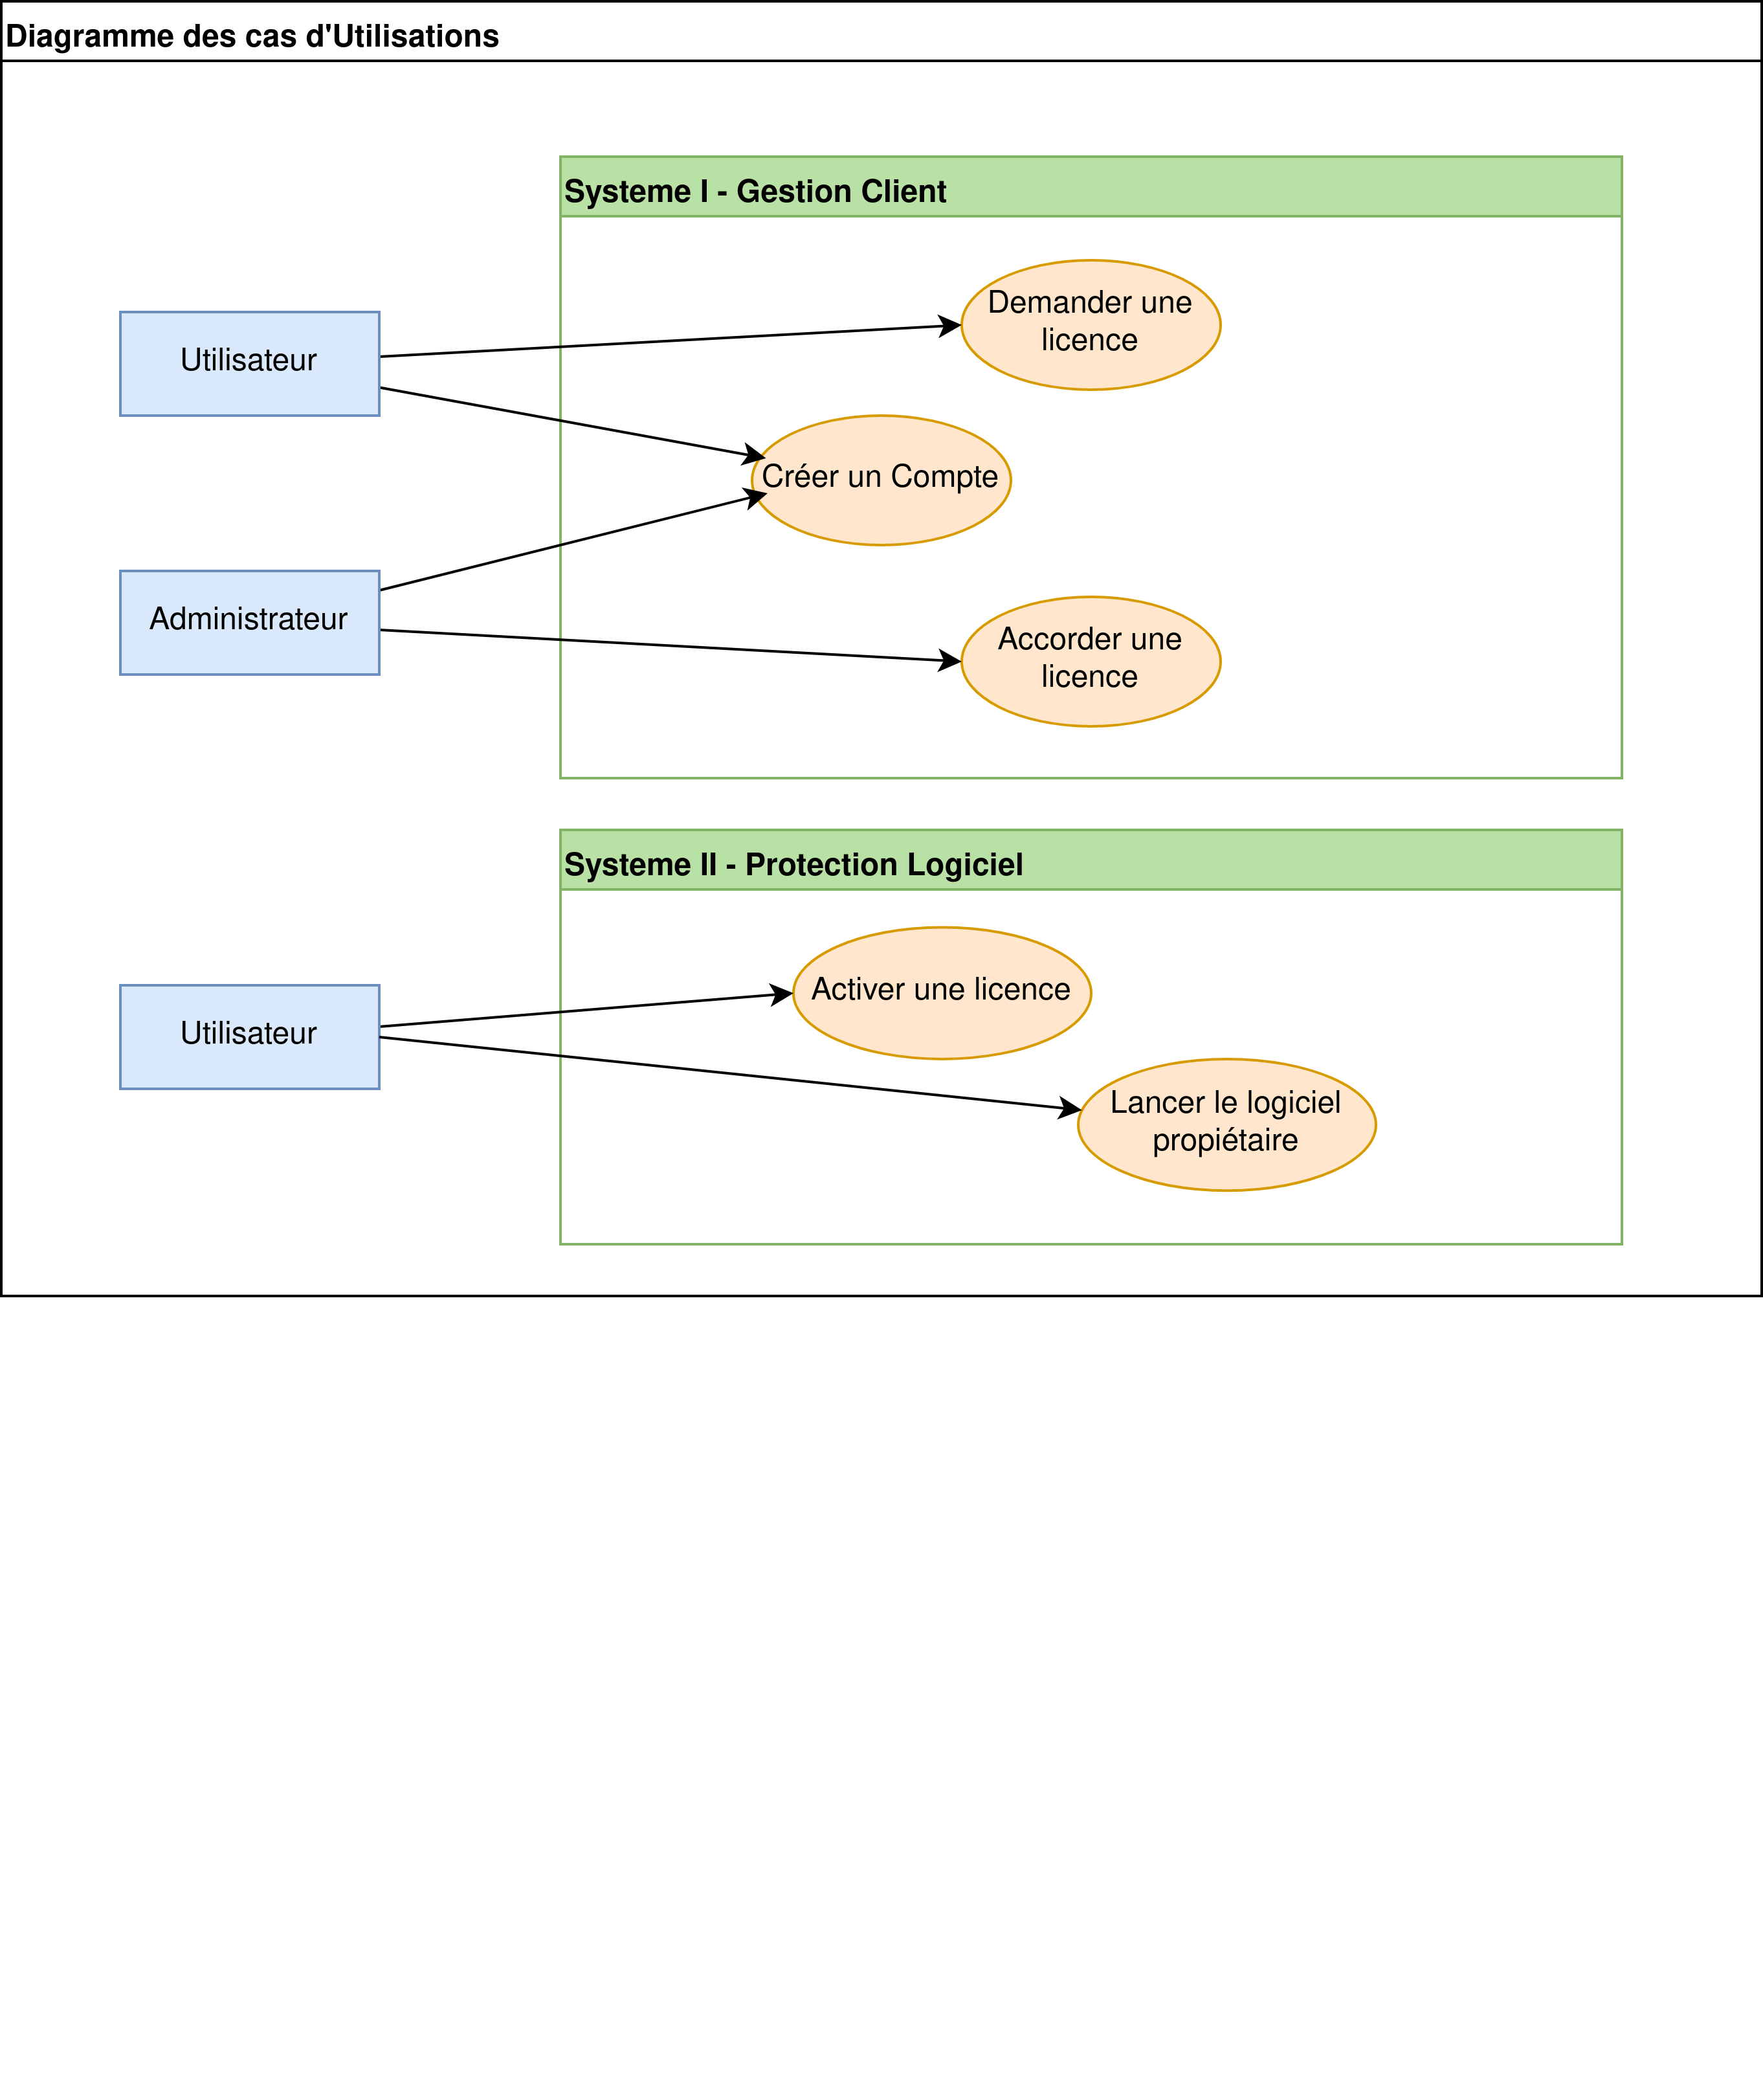
\includegraphics[scale=0.5]{img/Util.png}
    \end{figure}
\end{frame}

\begin{frame}{Exigences}
    \begin{itemize}
        \item Sécurité
        \pause
        \item Maintenabilité
        \pause
        \item Compatibilité Windows
    \end{itemize}
\end{frame}

%    \begin{tikzpicture}
%        \draw (0,0) ellipse (1.5cm and 0.5cm) node[black,fill=white]{Chiffrement};
%        \draw (3,0) ellipse (1.5cm and 0.5cm) node[black,fill=white]{PBKDF};
%        \draw (7,0) ellipse (1.8cm and 0.5cm) node[black,fill=white]{Base de données};
%        \draw (11,0) ellipse (1.5cm and 0.5cm) node[black,fill=white]{Obfuscation};
%    \end{tikzpicture}
%    \begin{tikzpicture}
%        \draw (5,0) ellipse (1.8cm and 0.5cm) node[black,fill=white]{Documentation};
%        \draw (10,0) ellipse (1.8cm and 0.5cm) node[black,fill=white]{Charte de code};
%    \end{tikzpicture}
%     \begin{tikzpicture}
%        \draw (3,0) ellipse (2cm and 0.5cm) node[black,fill=white]{Tests sur Windows};
%        \draw (7,0) ellipse (1.2cm and 0.5cm) node[black,fill=white]{DLL};
%        \draw (10,0) ellipse (1.5cm and 0.5cm) node[black,fill=white]{Injection PE};
%    \end{tikzpicture}

\begin{frame}{Fonctionnement globale}
    \begin{figure}
        \centering
        \vspace{-0.1cm}
        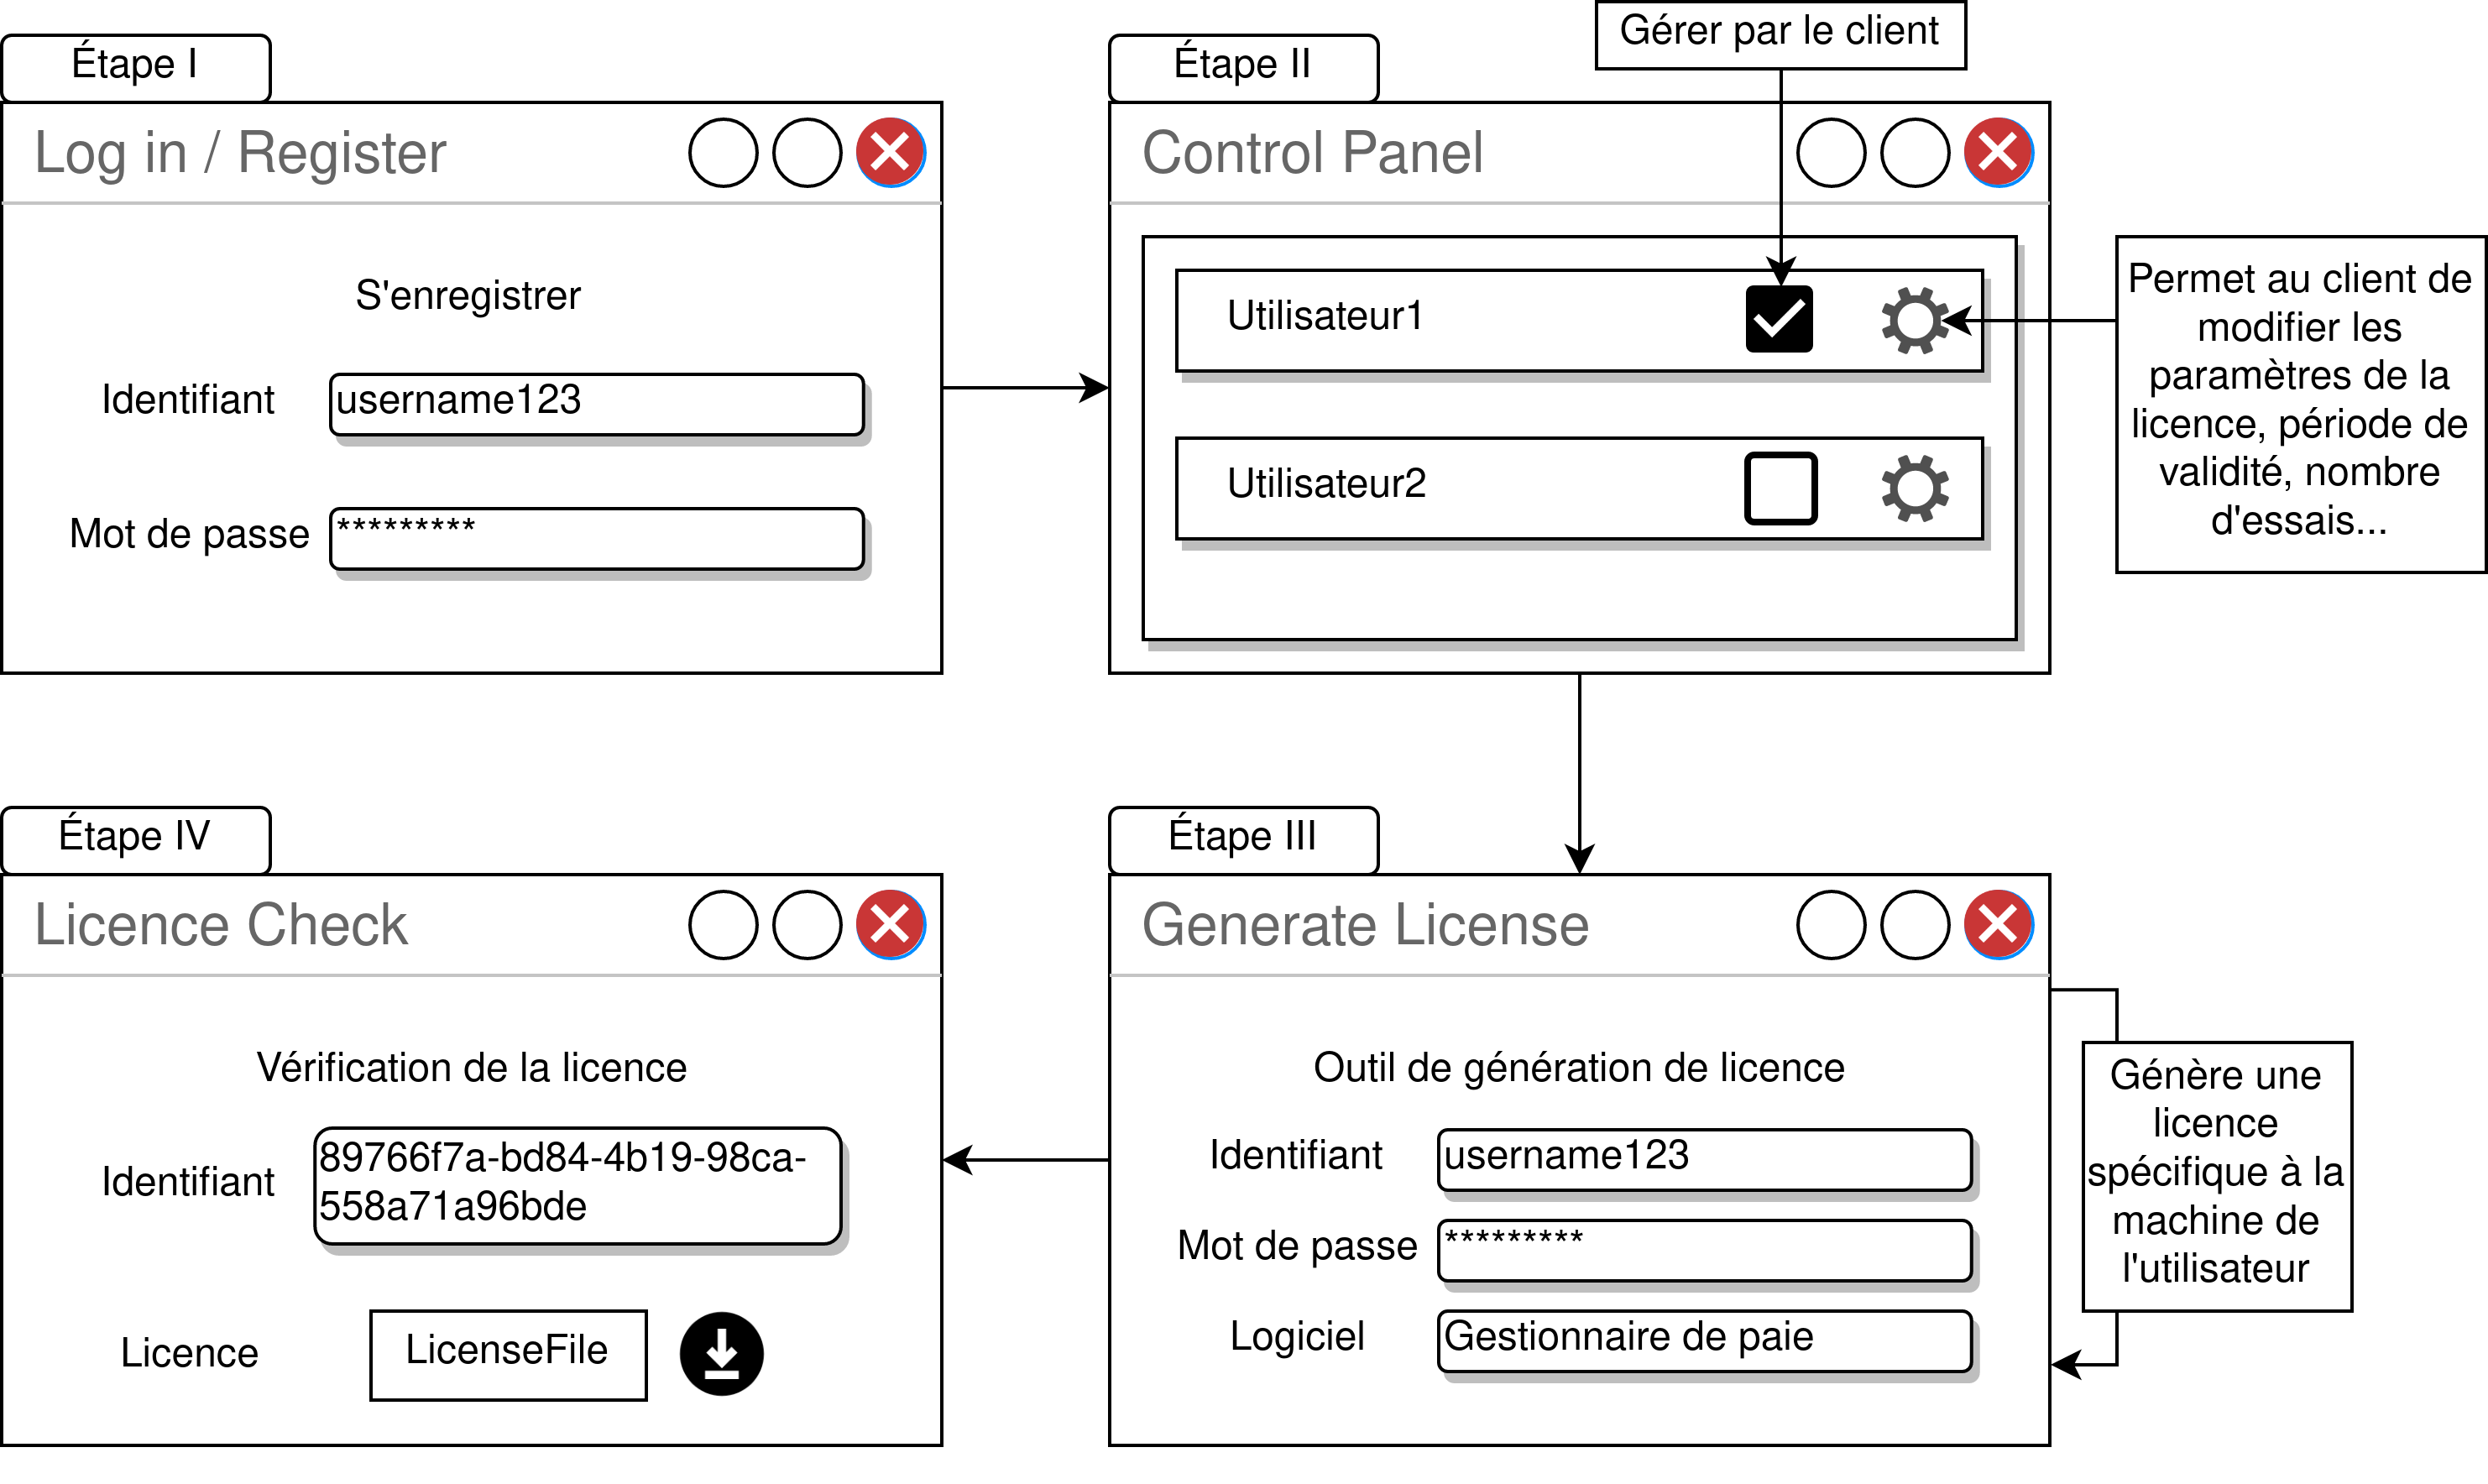
\includegraphics[scale=0.58]{img/STB.png}
    \end{figure}
\end{frame}

\section{Solution technique}

\begin{frame}{Architecture logicielle - Serveur}
    \begin{figure}
        \centering
        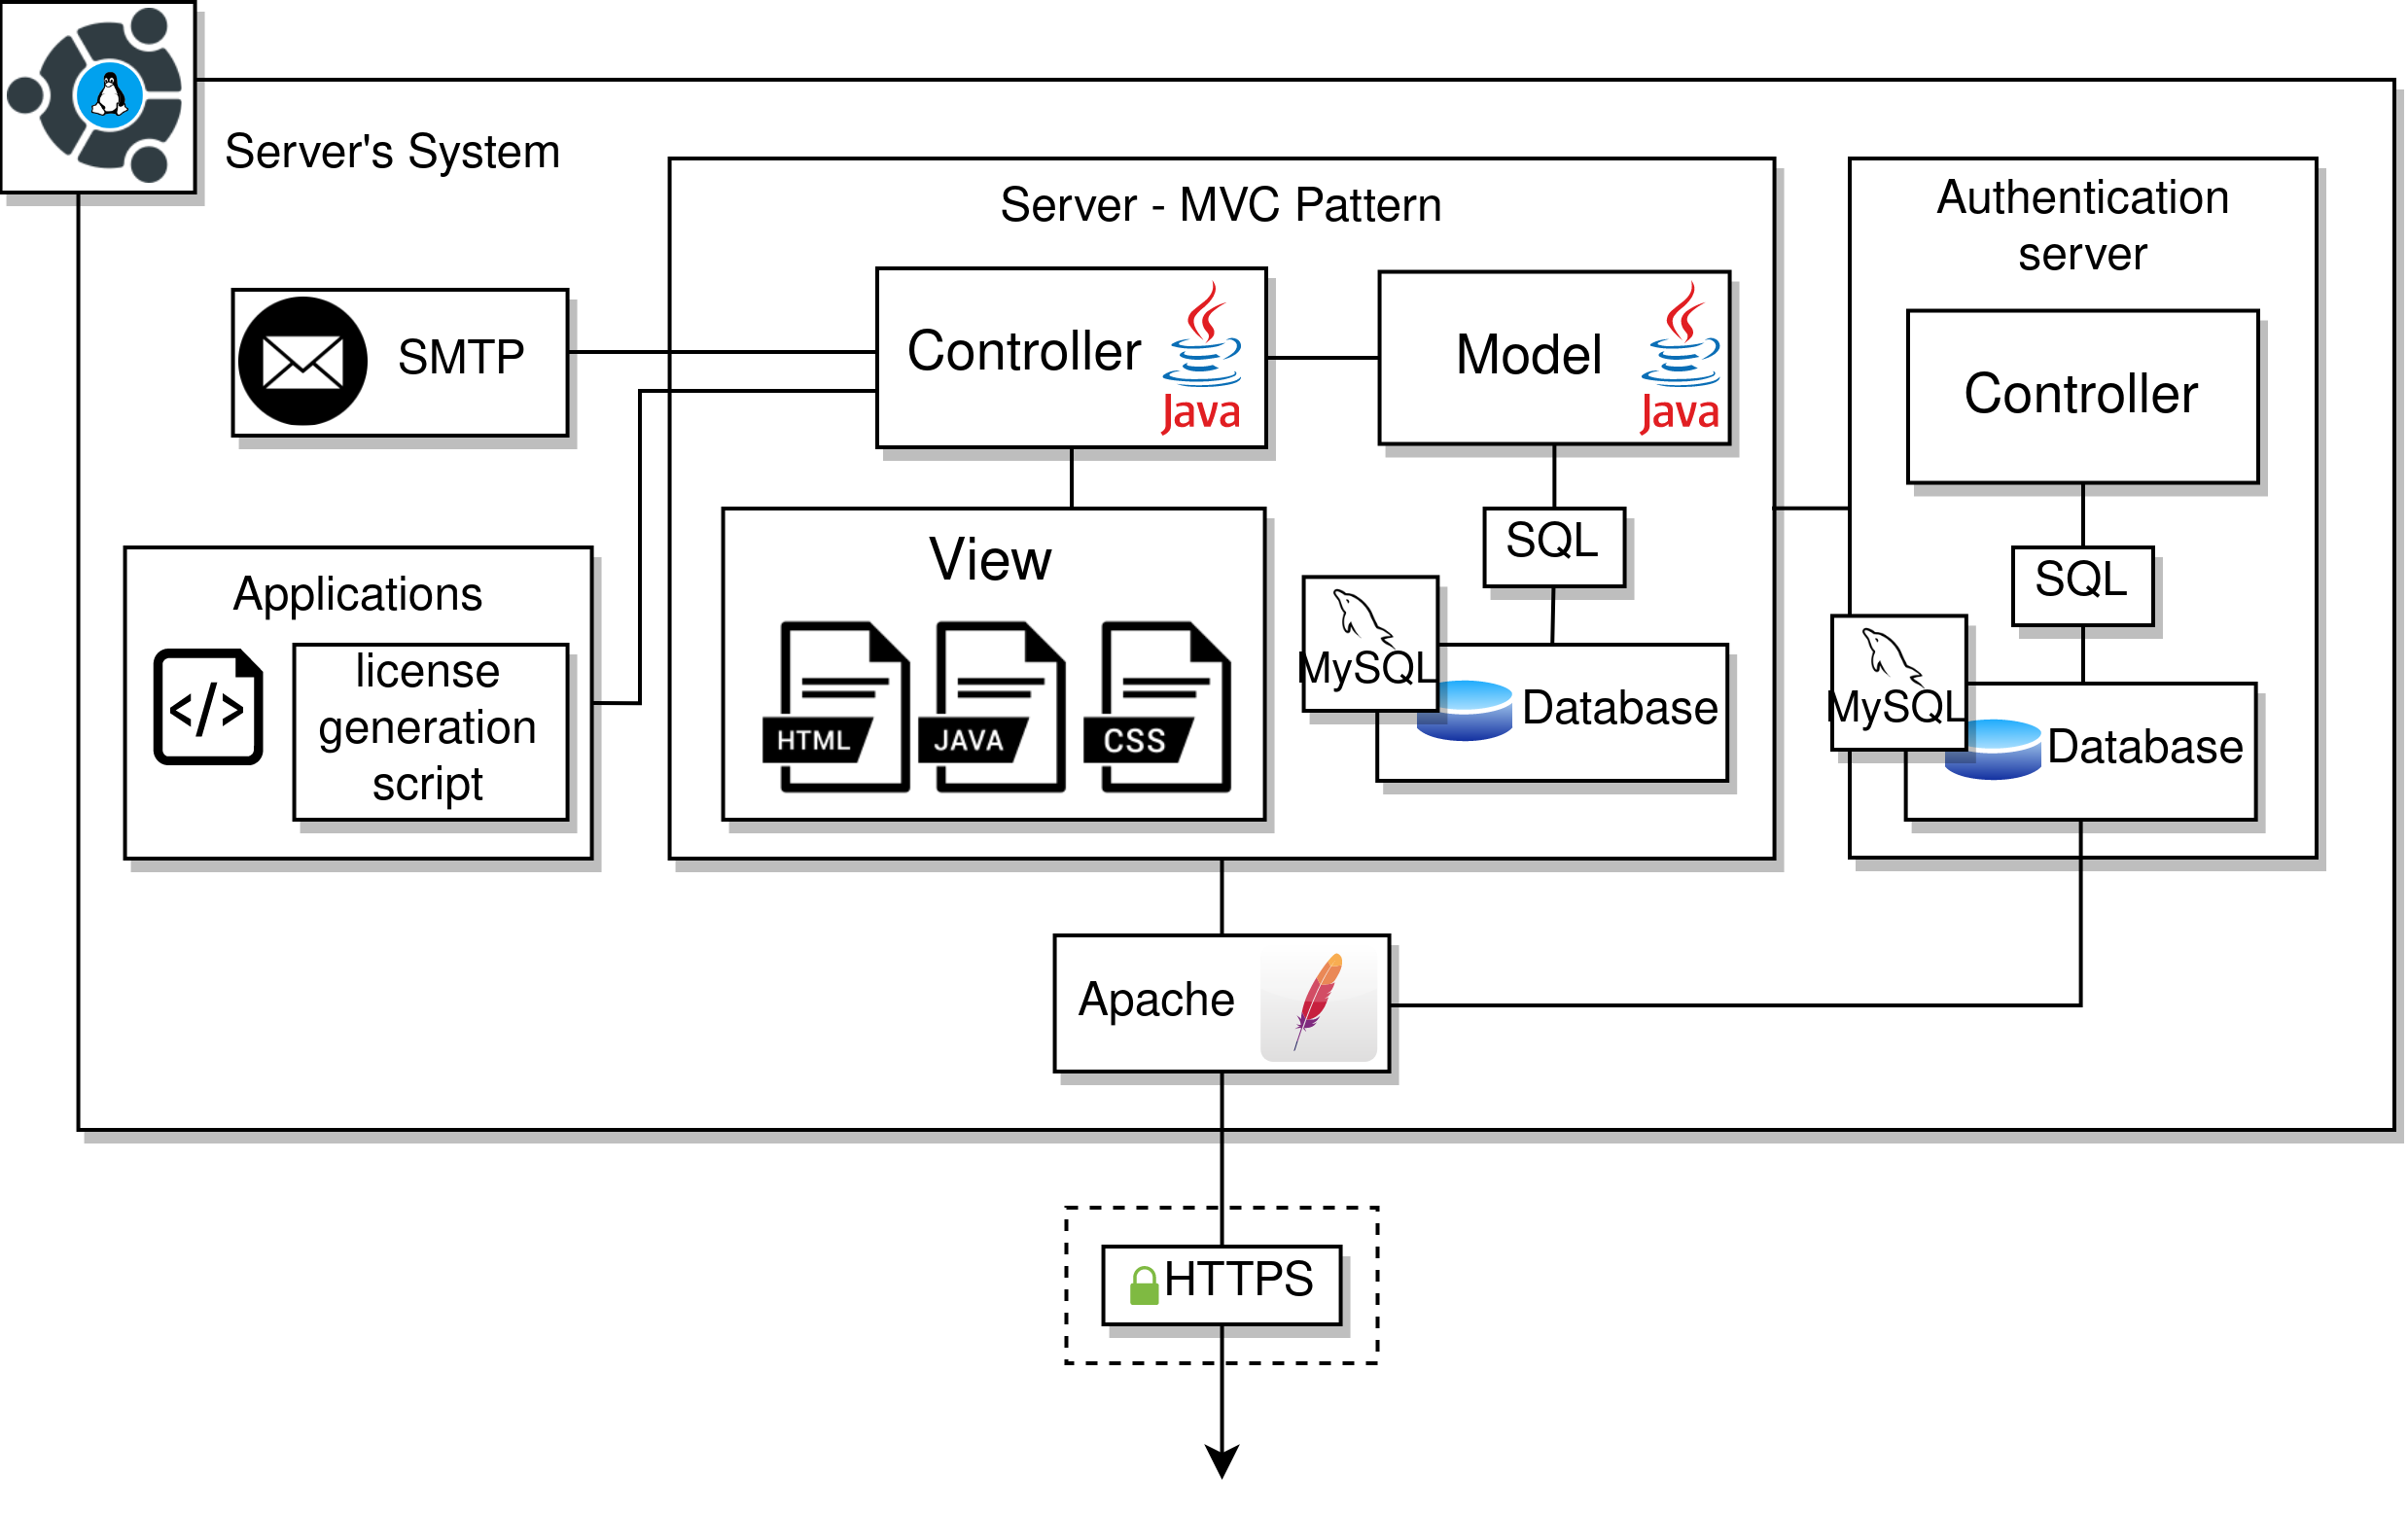
\includegraphics[scale=0.7]{img/DAT-server.png}
    \end{figure}
\end{frame}

\begin{frame}{Architecture logicielle - Client}
    \begin{figure}
        \centering
        \vspace{-0.8cm}
        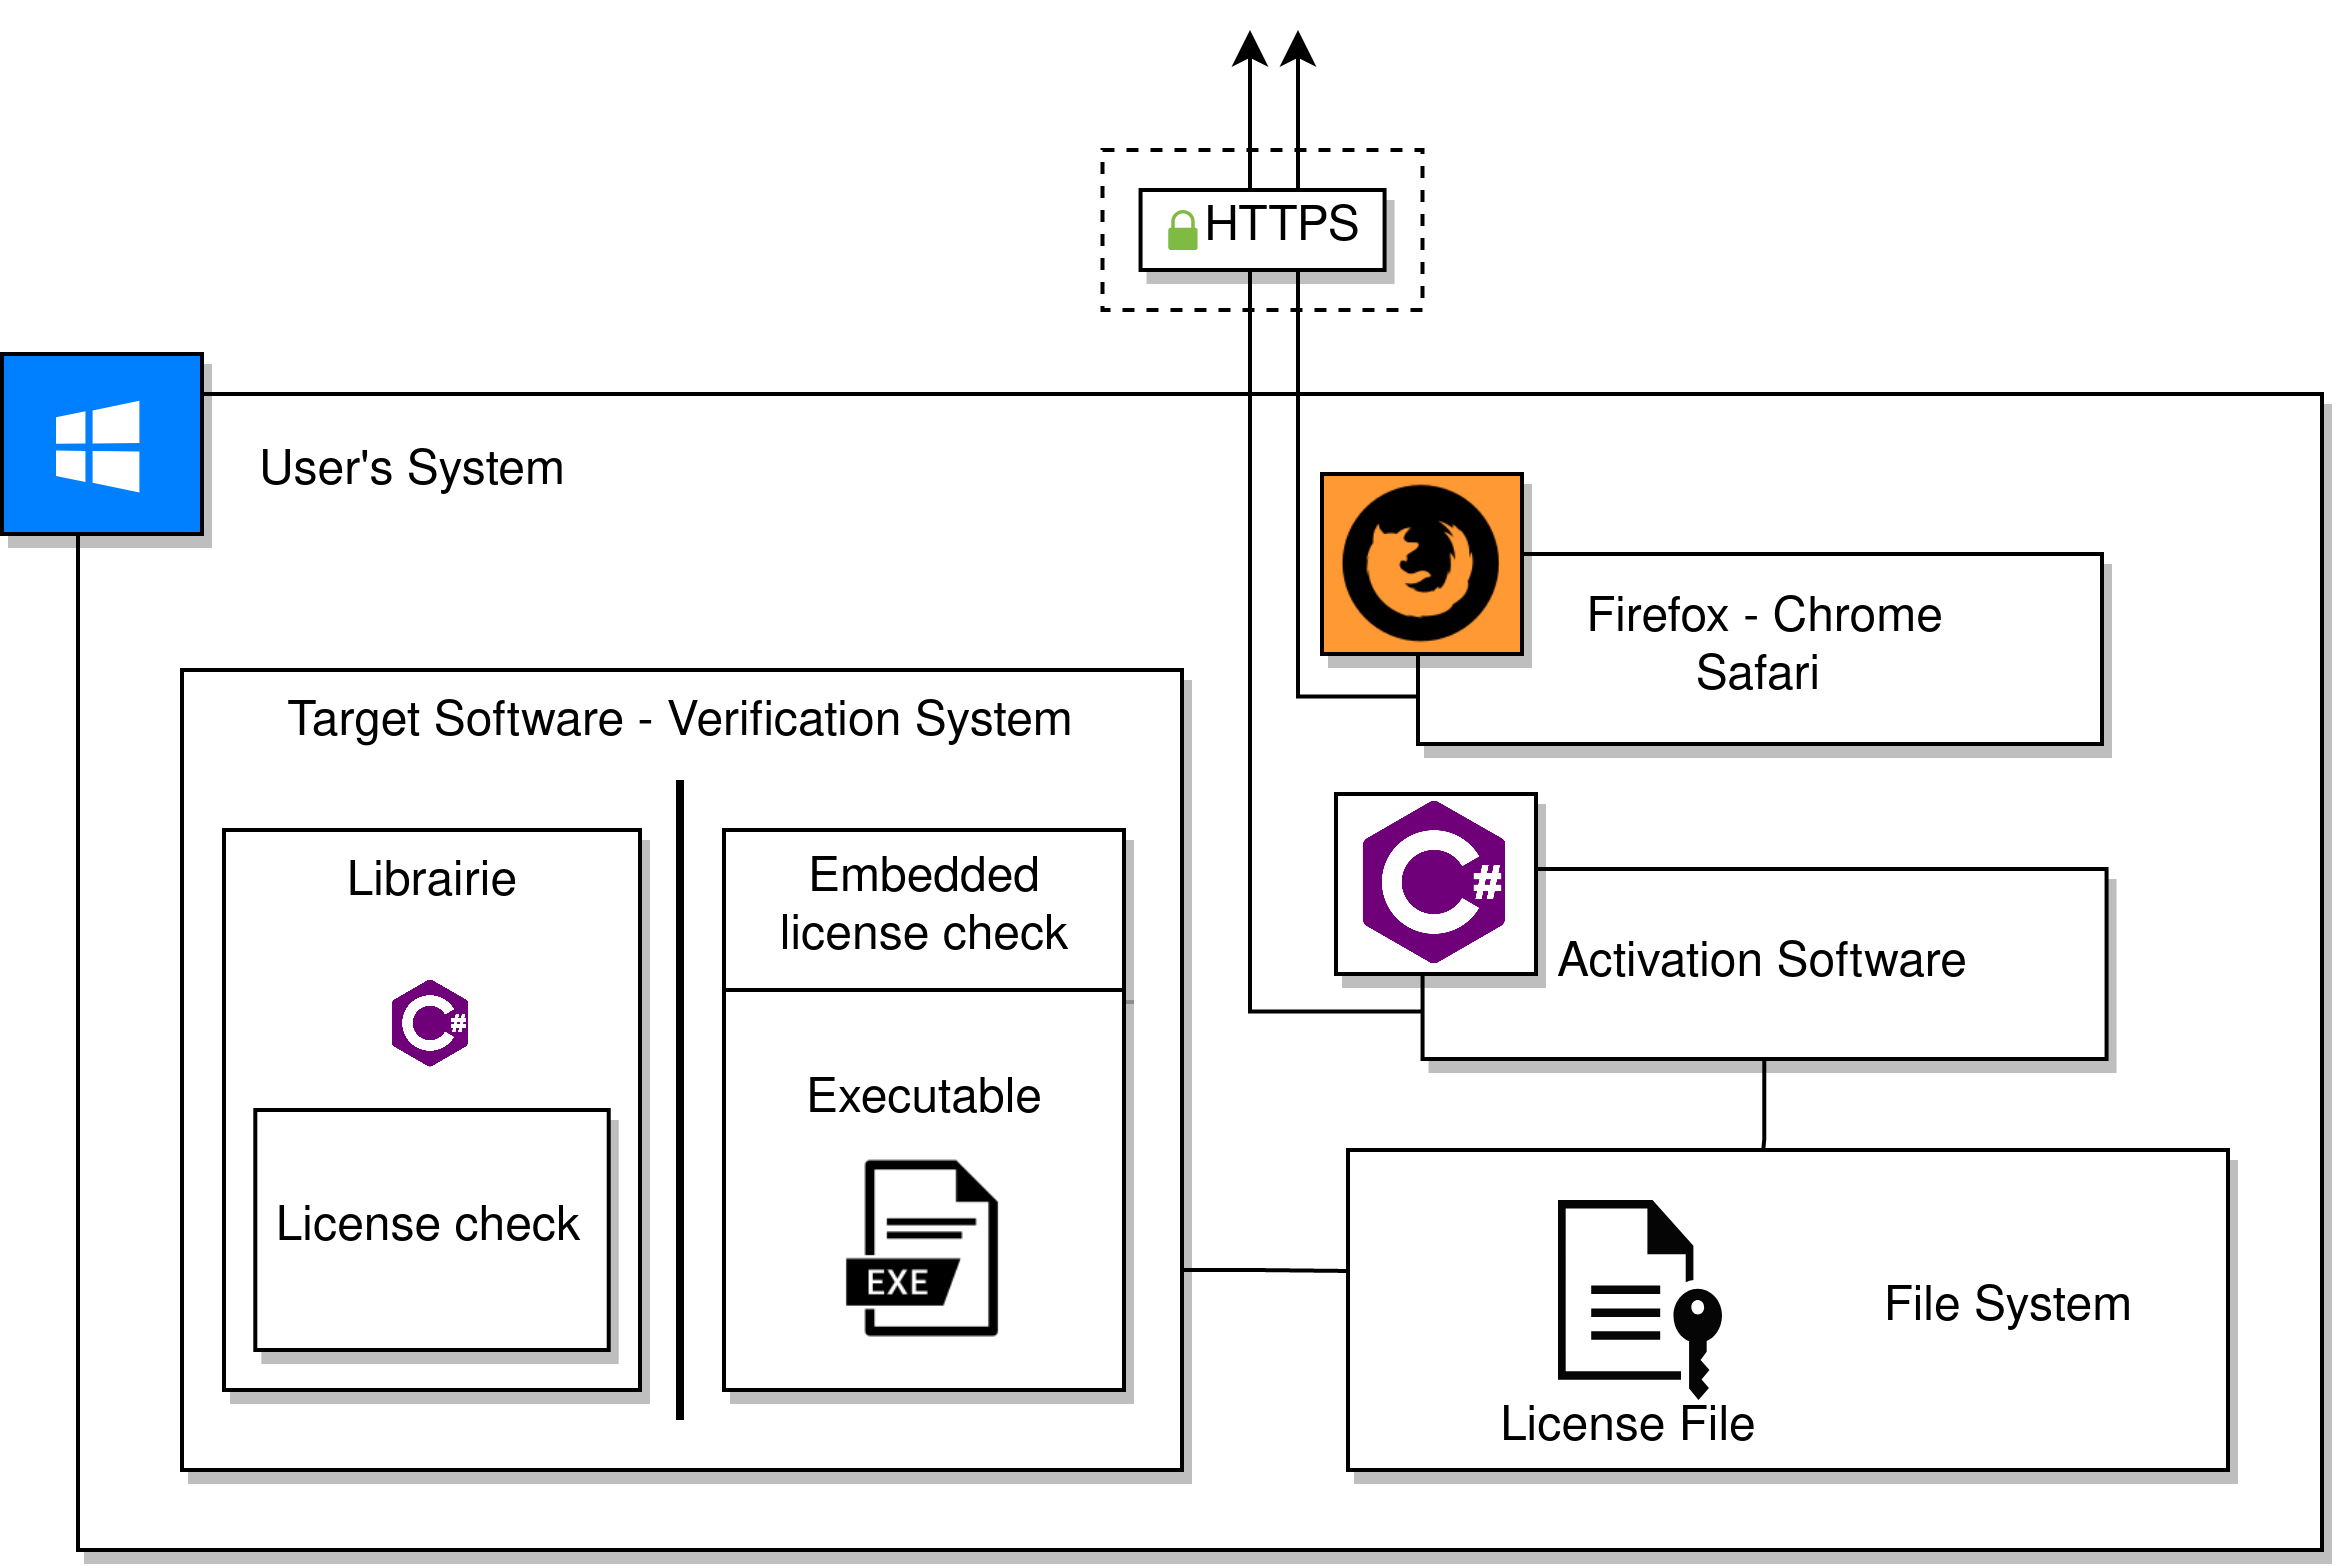
\includegraphics[scale=0.72]{img/DAT-client.png}
    \end{figure}
\end{frame}

\begin{frame}{Solutions techniques}
    Solutions apportées en réponse aux exigences techniques :
    \begin{description}
        \item[Plateforme sûre : ] chiffrement, serveur d'authentification, PBKDF,
            sécurisation des bases de données, API Rest avec utilisation de tokens
        \item[Génération et vérification de licence : ] signature (El Gamal), obfuscation
        \item[Maintenabilité : ] documentation, charte de code
    \end{description}
\end{frame}    

\section{Risques}

\begin{frame}{Risques principaux}
    \begin{itemize}
        \item Minimiser les failles de sécurité
            \begin{itemize}
                \item Configuration de la BDD
                \item Requêtes préparées
                \item Chiffrement/hashage des données
                \item Serveur d'authentification isolée (configuration)
            \end{itemize}
        \item Injection dans un PE
        \item Protéger le produit final par l'obfuscation
    \end{itemize}
\end{frame}

\section{Stratégie qualité} % en réponse aux risques

\begin{frame}{Actions à mettre en place}
    \begin{itemize}
        \item Gestion des anomalies et journalisation des bugs : MantisBT
        \item Tests d'intrusion
        \item Serveur de tests
        \item Jupiter (tests unitaires sur le modèle Java)
    \end{itemize}
\end{frame}

\section{Organisation du projet} % + planning

\begin{frame}{Affectation des rôles}
    \begin{figure}
        \centering
        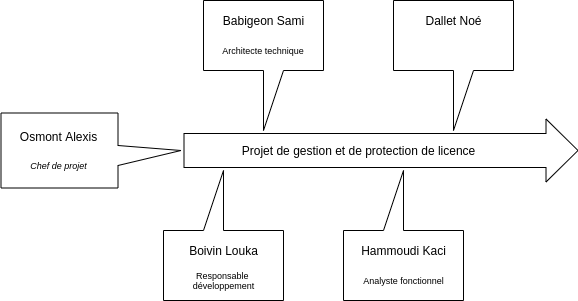
\includegraphics[scale=0.55]{img/schema_role_projet.png}
    \end{figure}
\end{frame}

\begin{frame}{Découpage des tâches}
    \begin{figure}
        \centering
        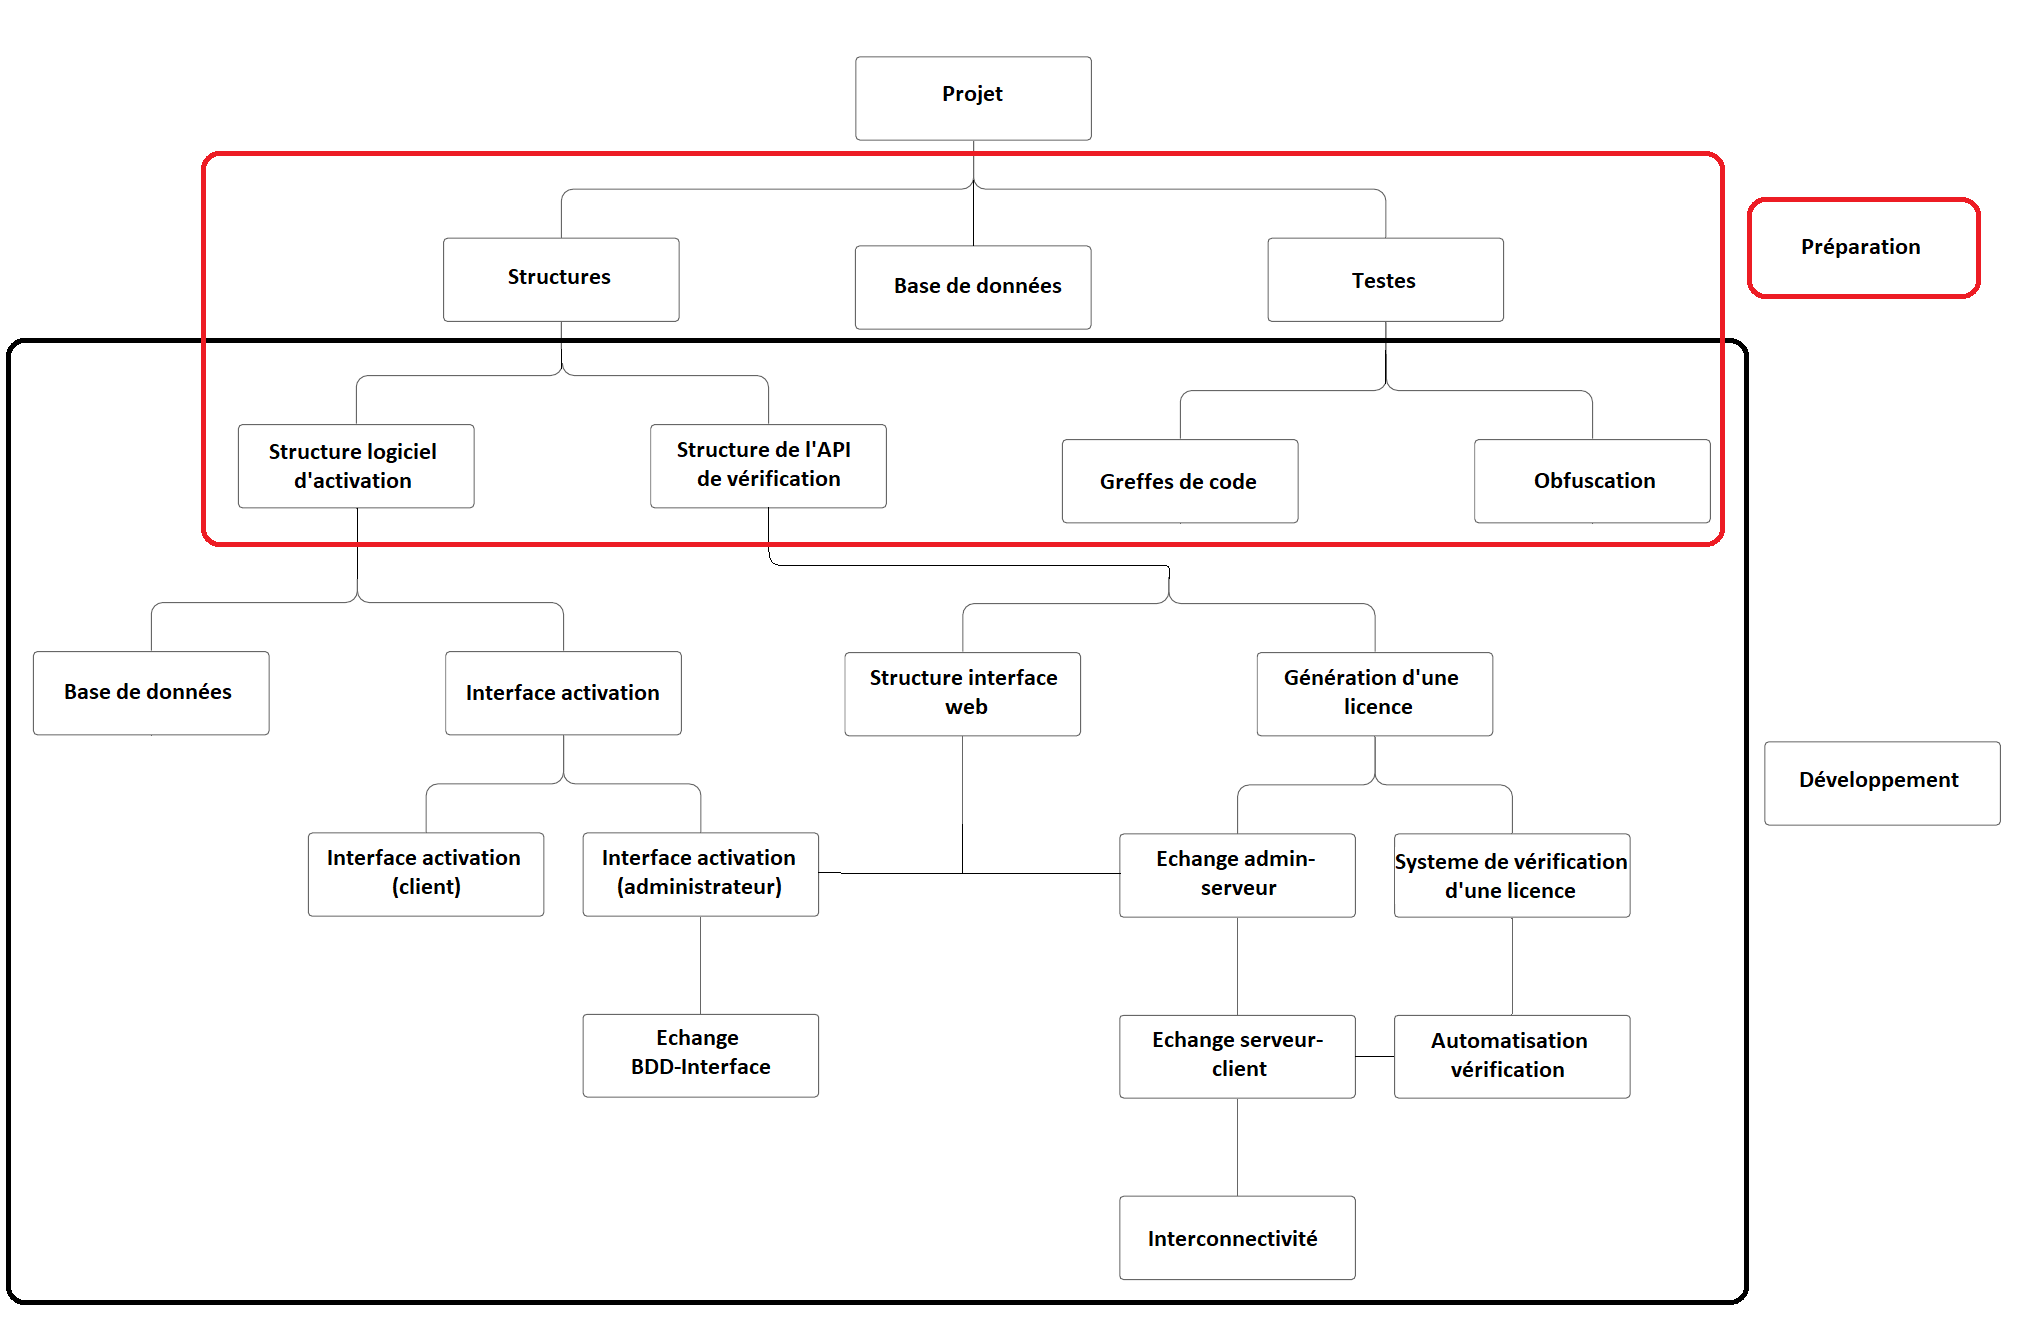
\includegraphics[scale=0.18]{img/organi.png}
    \end{figure}
\end{frame}

\begin{frame}{Diagramme de Gantt}
    \begin{figure}
        \centering
        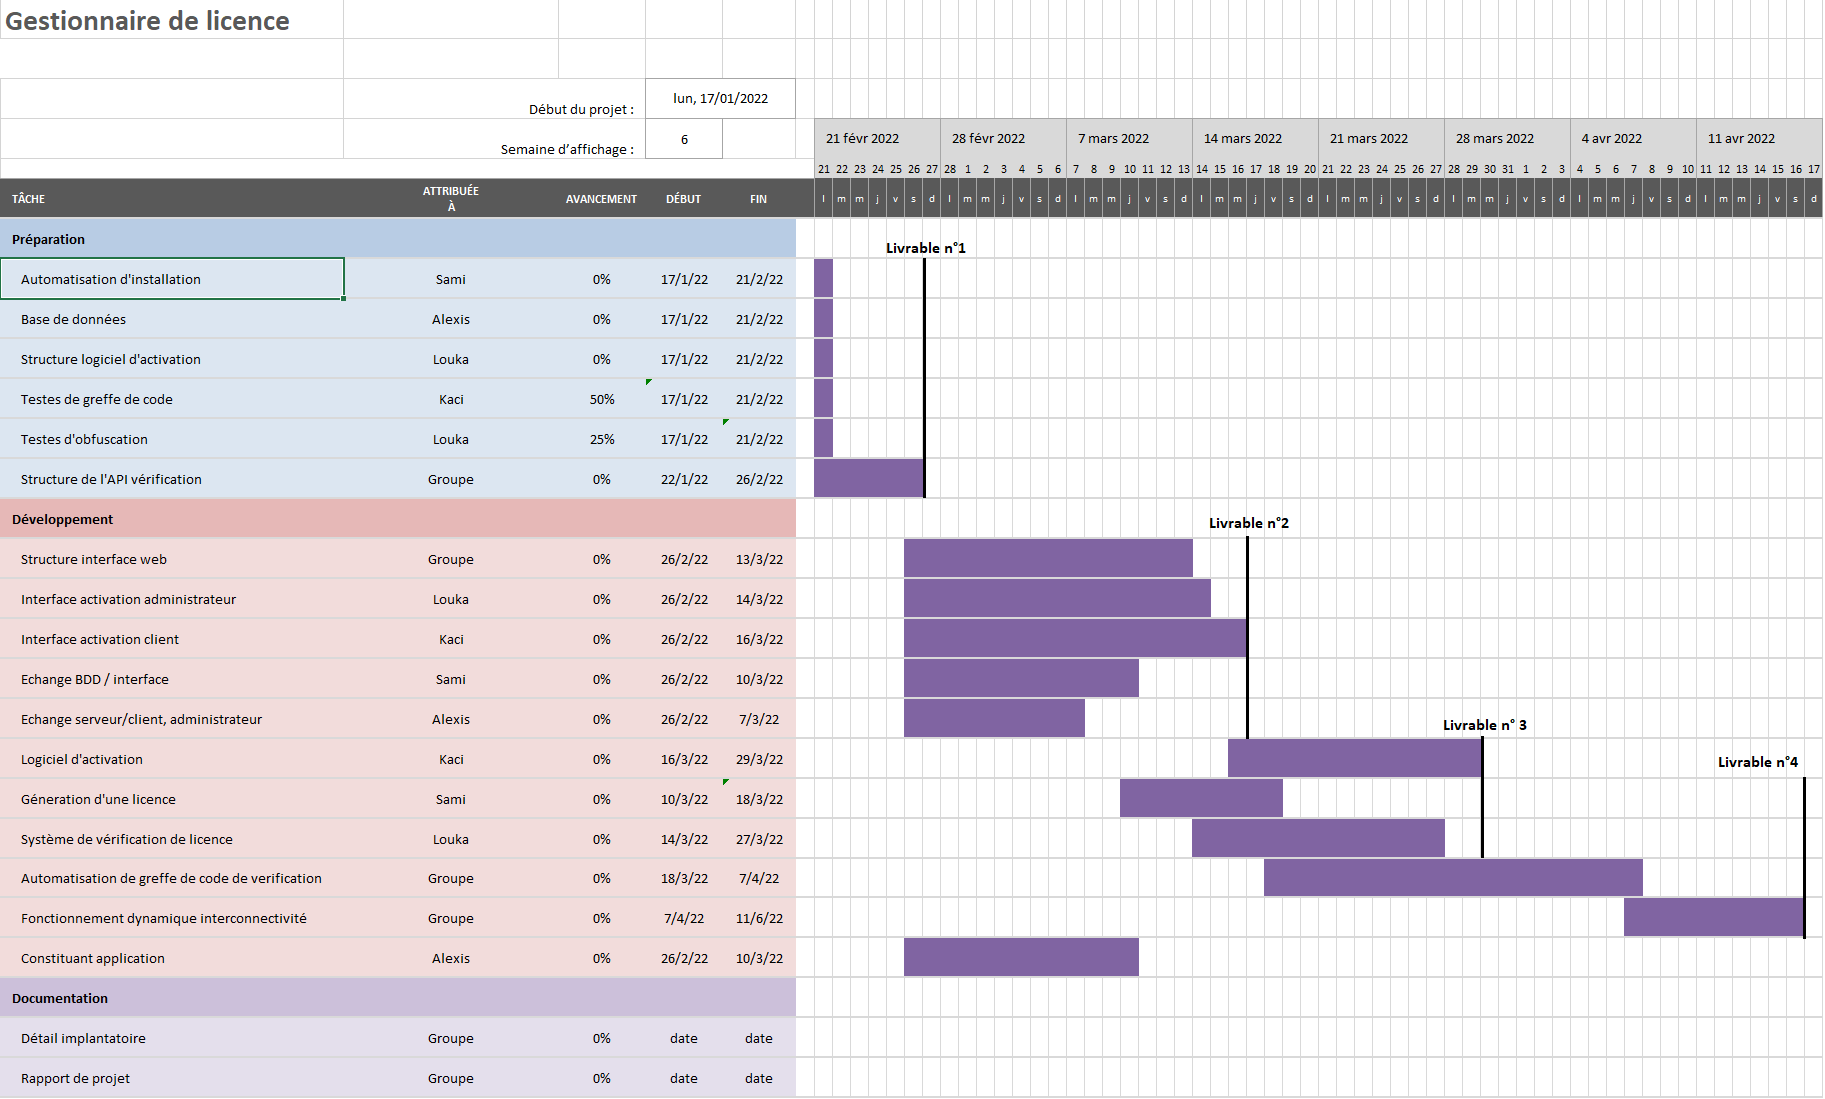
\includegraphics[scale=0.22]{img/Gantt.png}
    \end{figure}
\end{frame}

% Q&A
\begin{frame}[standout]
    \Huge\textsc{Merci de votre écoute}
    \vfill
    \LARGE\textsc{Questions ?}
\end{frame}

\end{document}

